% !TeX program = xelatex
% !BIB program = biber
% CPUT Thesis Template
% LaTeX version of CPUT Thesis Template Word document
% Compile with PDFLaTeX, XeLaTeX, or LuaLaTeX

\documentclass{cputthesis}

\addbibresource{references.bib}

% Thesis metadata - fill these in
\thesistitle{TITLE OF THESIS/DISSERTATION}
\authorfull{FULL FIRST NAMES \& SURNAME}
\degreetype{Master of Technology/Doctor of Technology: (choose one)}
\discipline{Discipline (e.g. Chemical Engineering, Public Relations Management)}
\faculty{in the Faculty of (name of Faculty)}
\supervisor{Supervisor: Type the name of your supervisor here, e.g. Prof BA Brain}
\cosupervisor{Co-supervisor: Add if necessary -- otherwise delete}
\campus{Bellville/Cape Town/Mowbray/Wellington (choose campus)}
\submissiondate{Date submitted (e.g. September 2007)}

\begin{document}

% Title page
\maketitle

% Declaration
\begin{declaration}
I, type your full first names and surname here, declare that the contents of this dissertation/thesis represent my own unaided work, and that the dissertation/thesis has not previously been submitted for academic examination towards any qualification. Furthermore, it represents my own opinions and not necessarily those of the Cape Peninsula University of Technology.
\end{declaration}

% Abstract
\begin{cputabstract}
Type your Abstract here in 1½-line spacing. Length: 1-2 pages maximum, preferably 1 page.
\end{cputabstract}

% Acknowledgements
\begin{acknowledgements}
\textbf{I wish to thank:}

\begin{itemize}
\item Type name of person here, with brief explanation if necessary.
\item Type name of person here, with brief explanation if necessary.
\item Type name of person here, with brief explanation if necessary.
\item Type name of person here, with brief explanation if necessary. Use as many bullets as you wish (but within reason).
\end{itemize}

\textbf{If you have received funding from the NRF, include the following:}

The financial assistance of the National Research Foundation towards this research is acknowledged. Opinions expressed in this thesis and the conclusions arrived at, are those of the author, and are not necessarily to be attributed to the National Research Foundation.
\end{acknowledgements}

% Dedication (optional)
\begin{dedication}
This is optional, and may be omitted.

\vspace{1cm}

For (whomever)
\end{dedication}

% Manual template table of contents and lists, matching the Word template.
% Replace with \tableofcontents, \listoffigures, and \listoftables if your
% department asks for generated lists.
\cputmanualcontents

% Glossary (if needed)
\begin{cputglossary}
\textbf{List any terms, acronyms or abbreviations (with the appropriate caption) used here. Use single-line spacing, with a line between each item.}

\noindent\begin{tabularx}{0.96\textwidth}{|Y|Y|}
\hline
\textbf{Terms/Acronyms/Abbreviations} & \textbf{Definition/Explanation} \\
\hline
 & \\[1.2\baselineskip]
 & \\[1.2\baselineskip]
 & \\[1.2\baselineskip]
 & \\[1.2\baselineskip]
 & \\[1.2\baselineskip]
\hline
\end{tabularx}
\end{cputglossary}

\mainmatter

% Chapters
% Each chapter can be in a separate file and included with % Chapter 1

\chapter{TYPE THE TITLE OF THE CHAPTER HERE}

\section{Introduction}

Ensure that MsWord is set and defaulted to English (UK) or English (SA). Your margins should be 3cm (left) (as this allows for binding) and 2cm (right, top and bottom). Type your dissertation/thesis for all chapters in 1½-line spacing, 11-point. (Items in the Bibliography and information typed inside tables are typed in single-line spacing.) Use \underline{one space} after all punctuation marks. Use decimal subdivisions as indicated below. Consult \textcite{van-aswegen-2006} for information on research writing and bibliographic style. The collation of the thesis is also discussed at length \parencite[33]{van-aswegen-2006}. Note the use of the Harvard style of bibliographic citation. Footnotes should be used sparingly (use Microsoft Word: Insert -- Reference -- Footnote), mainly to clarify concepts or add information which does not pertain directly to the text.\footnote{Candidates writing a thesis or dissertation will find helpful manuals in the CPUT library at DDC number 808.02.} Note the justified right-hand margin in the text. NB. Do \underline{not justify right} tables or the Bibliography/References, as this will give you unnecessary white space. Press enter twice to move to the next paragraph.

Two authors in running text: \textcite{ellis-peters-2000} argue that literature is important (Ellis and Peters, 2000:45).

Two authors in parentheses: \parencite[45]{ellis-peters-2000}.

Three or more authors: \textcite{henderson-etal-1987} claim that moral philosophy is fundamental (Henderson et al., 1987:12).

\subsection{Heading: use sentence case, as in this example}

\subsection{Heading}

\subsubsection{Heading}

\subsubsection{Heading}

% Example figure
\begin{figure}[htbp]
\centering
% \includegraphics[width=0.8\textwidth]{example-image}
\caption{Add caption \underline{below} the figure (10-point bold)}
\label{fig:1.1}
\end{figure}

\textbf{Use single-line spacing and sentence case with no full stop}

\textbf{Centre, or align left}

\textbf{(Adapted from Bloggs, 1999:34)}

% Example table
\begin{table}[htbp]
\centering
\caption{Add caption \underline{above} the table (10-point bold), single-line spacing, sentence case, and no full stop}
\begin{tabularx}{\textwidth}{|Y|Y|Y|Y|>{\raggedleft\arraybackslash}p{1.8cm}|}
\hline
\textbf{Heading} & \textbf{Heading} & \textbf{Heading} & \textbf{Heading} & \textbf{Rands} \\
\hline
Remember to justify left and use single spacing. Check your punctuation at the end and be consistent. & Use a smaller font if you have a great deal of text. This is 9-point Arial. & Eight-point is generally too small to be read comfortably. & Use right justification for figures, as in the next table. Remember to right align the caption, also. & 1 234 \\
\hline
130 & 18 987 & 120 764 & 123 & \\
\hline
Text of tables should not ``overflow'' onto the next page, but should be enclosed in a new row and column. & Very wide tables should be ``landscaped'' -- remember to use a wide-enough margin for binding. & & & \\
\hline
\end{tabularx}
\label{tab:1.1}
\end{table}

\textbf{Equations}

\begin{equation}
\label{eq:1.1}
E = mc^2
\end{equation}
See Equation~\ref{eq:1.1}.

% or written directly here

% Chapter 1

\chapter{TYPE THE TITLE OF THE CHAPTER HERE}

\section{Introduction}

Ensure that MsWord is set and defaulted to English (UK) or English (SA). Your margins should be 3cm (left) (as this allows for binding) and 2cm (right, top and bottom). Type your dissertation/thesis for all chapters in 1½-line spacing, 11-point. (Items in the Bibliography and information typed inside tables are typed in single-line spacing.) Use \underline{one space} after all punctuation marks. Use decimal subdivisions as indicated below. Consult \textcite{van-aswegen-2006} for information on research writing and bibliographic style. The collation of the thesis is also discussed at length \parencite[33]{van-aswegen-2006}. Note the use of the Harvard style of bibliographic citation. Footnotes should be used sparingly (use Microsoft Word: Insert -- Reference -- Footnote), mainly to clarify concepts or add information which does not pertain directly to the text.\footnote{Candidates writing a thesis or dissertation will find helpful manuals in the CPUT library at DDC number 808.02.} Note the justified right-hand margin in the text. NB. Do \underline{not justify right} tables or the Bibliography/References, as this will give you unnecessary white space. Press enter twice to move to the next paragraph.

Two authors in running text: \textcite{ellis-peters-2000} argue that literature is important (Ellis and Peters, 2000:45).

Two authors in parentheses: \parencite[45]{ellis-peters-2000}.

Three or more authors: \textcite{henderson-etal-1987} claim that moral philosophy is fundamental (Henderson et al., 1987:12).

\subsection{Heading: use sentence case, as in this example}

\subsection{Heading}

\subsubsection{Heading}

\subsubsection{Heading}

% Example figure
\begin{figure}[htbp]
\centering
% \includegraphics[width=0.8\textwidth]{example-image}
\caption{Add caption \underline{below} the figure (10-point bold)}
\label{fig:1.1}
\end{figure}

\textbf{Use single-line spacing and sentence case with no full stop}

\textbf{Centre, or align left}

\textbf{(Adapted from Bloggs, 1999:34)}

% Example table
\begin{table}[htbp]
\centering
\caption{Add caption \underline{above} the table (10-point bold), single-line spacing, sentence case, and no full stop}
\begin{tabularx}{\textwidth}{|Y|Y|Y|Y|>{\raggedleft\arraybackslash}p{1.8cm}|}
\hline
\textbf{Heading} & \textbf{Heading} & \textbf{Heading} & \textbf{Heading} & \textbf{Rands} \\
\hline
Remember to justify left and use single spacing. Check your punctuation at the end and be consistent. & Use a smaller font if you have a great deal of text. This is 9-point Arial. & Eight-point is generally too small to be read comfortably. & Use right justification for figures, as in the next table. Remember to right align the caption, also. & 1 234 \\
\hline
130 & 18 987 & 120 764 & 123 & \\
\hline
Text of tables should not ``overflow'' onto the next page, but should be enclosed in a new row and column. & Very wide tables should be ``landscaped'' -- remember to use a wide-enough margin for binding. & & & \\
\hline
\end{tabularx}
\label{tab:1.1}
\end{table}

\textbf{Equations}

\begin{equation}
\label{eq:1.1}
E = mc^2
\end{equation}
See Equation~\ref{eq:1.1}.

% Chapter 2

\chapter{Literature review}

\section{Literature Review Introduction}

Starting of text

\begin{itemize}
\item Bullet (single spacing)
\item Bullet
\item Bullet
\end{itemize}

Figures comprise photographs, diagrams, graphs, bar charts, pie charts, etc. They are all termed ``Figures'', and are captioned \underline{below the figure} (Microsoft Word: Insert -- Reference -- Caption). If the caption is longer than one line, it should be typed in \underline{single line-spacing}. Figures taken (or adapted) from a source should be acknowledged as in the example below, and should appear in the Bibliography/References. Leave at least two spaces (press enter twice) above and below a figure, to separate it from the text.

% Example figure
\begin{figure}[htbp]
\centering
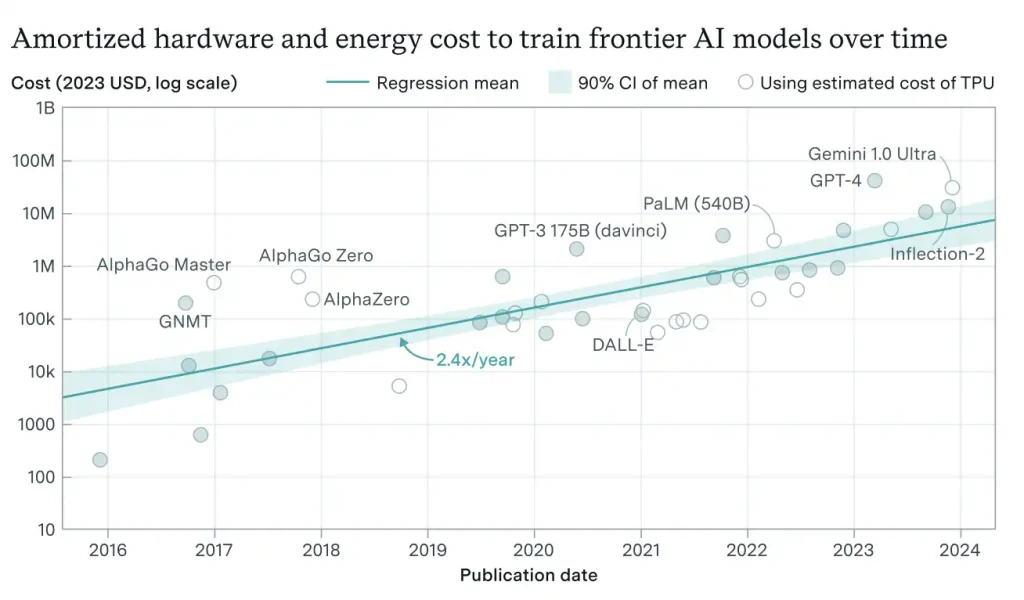
\includegraphics[width=0.8\textwidth]{media/Fig1.png}
\caption{Example figure}
\label{fig:2.1}
\end{figure}

Tables comprise text and figures in tabular form. Tables are typed in single line-spacing, with left justification. Figures should be aligned to the right, as in the example below. If you have a great deal of text, use a smaller (but legible) font, e.g. 9- or 10-point. Acknowledge tables taken from another source as for figures, above. Leave at least two spaces (press enter twice) above and below a table, to separate it from the text.

% Example table
\begin{table}[htbp]
\centering
\caption{Example table}
\begin{tabularx}{0.86\textwidth}{|Y|Y|Y|Y|>{\raggedleft\arraybackslash}p{1.8cm}|}
\hline
\textbf{Column 1} & \textbf{Column 2} & \textbf{Column 3} & \textbf{Column 4} & \textbf{Value} \\
\hline
Data 1 & Data 2 & Data 3 & Data 4 & 123.45 \\
\hline
Data 5 & Data 6 & Data 7 & Data 8 & 678.90 \\
\hline
\end{tabularx}
\label{tab:2.1}
\end{table}

% Chapter 3

\chapter{Methodology}

\section{Reinforcement learning formulation}

This synthetic chapter demonstrates how the template handles mathematical notation, displayed equations, aligned derivations, and multi-line optimisation objectives. The example frames a learning problem as a Markov decision process:

\begin{equation}
\mathcal{M} = \left(\mathcal{S}, \mathcal{A}, P, R, \gamma\right),
\label{eq:mdp}
\end{equation}

where $\mathcal{S}$ is the state space, $\mathcal{A}$ is the action space, $P(s' \mid s,a)$ is the transition probability, $R(s,a)$ is the expected reward, and $\gamma \in [0,1)$ is the discount factor. At each time step $t$, an agent observes a state $s_t$, selects an action $a_t \sim \pi_\theta(\cdot \mid s_t)$, receives reward $r_t$, and transitions to a new state $s_{t+1}$.

\section{Return and value functions}

The discounted return from time $t$ is defined as:

\begin{equation}
G_t = \sum_{k=0}^{\infty} \gamma^k r_{t+k+1}.
\label{eq:return}
\end{equation}

For a policy $\pi$, the state-value and action-value functions are:

\begin{align}
V^\pi(s) &= \mathbb{E}_\pi \left[ G_t \mid s_t = s \right], \label{eq:value}\\
Q^\pi(s,a) &= \mathbb{E}_\pi \left[ G_t \mid s_t = s, a_t = a \right]. \label{eq:qvalue}
\end{align}

The Bellman expectation equation expresses the recursive structure of $V^\pi$:

\begin{equation}
V^\pi(s) =
\sum_{a \in \mathcal{A}} \pi(a \mid s)
\sum_{s' \in \mathcal{S}} P(s' \mid s,a)
\left[R(s,a) + \gamma V^\pi(s')\right].
\label{eq:bellman-expectation}
\end{equation}

\section{Temporal-difference learning}

Temporal-difference learning updates value estimates by comparing current predictions with a bootstrapped target. The one-step temporal-difference error is:

\begin{equation}
\delta_t = r_{t+1} + \gamma V(s_{t+1}) - V(s_t).
\label{eq:td-error}
\end{equation}

A tabular value estimate can then be updated as:

\begin{equation}
V(s_t) \leftarrow V(s_t) + \alpha \delta_t,
\label{eq:td-update}
\end{equation}

where $\alpha$ is the learning rate. For action-value learning, the Q-learning update is:

\begin{equation}
Q(s_t,a_t) \leftarrow Q(s_t,a_t) +
\alpha \left[
r_{t+1} + \gamma \max_{a' \in \mathcal{A}} Q(s_{t+1},a') - Q(s_t,a_t)
\right].
\label{eq:q-learning}
\end{equation}

\section{Policy optimisation}

Policy-gradient methods optimise a parameterised policy by maximising the expected return:

\begin{equation}
J(\theta) = \mathbb{E}_{\tau \sim \pi_\theta}
\left[
\sum_{t=0}^{T} \gamma^t r_{t+1}
\right].
\label{eq:policy-objective}
\end{equation}

Using the likelihood-ratio identity, the gradient can be estimated as:

\begin{equation}
\nabla_\theta J(\theta) =
\mathbb{E}_{\tau \sim \pi_\theta}
\left[
\sum_{t=0}^{T}
\nabla_\theta \log \pi_\theta(a_t \mid s_t) A^\pi(s_t,a_t)
\right],
\label{eq:policy-gradient}
\end{equation}

where $A^\pi(s,a)$ is the advantage function:

\begin{equation}
A^\pi(s,a) = Q^\pi(s,a) - V^\pi(s).
\label{eq:advantage}
\end{equation}

For clipped policy optimisation, the probability ratio between the updated and previous policies is:

\begin{equation}
\rho_t(\theta) =
\frac{\pi_\theta(a_t \mid s_t)}
{\pi_{\theta_{\mathrm{old}}}(a_t \mid s_t)}.
\label{eq:ratio}
\end{equation}

The clipped surrogate objective is:

\begin{equation}
L^{\mathrm{clip}}(\theta) =
\mathbb{E}_t
\left[
\min\left(
\rho_t(\theta) A_t,\,
\operatorname{clip}\left(\rho_t(\theta), 1-\epsilon, 1+\epsilon\right) A_t
\right)
\right].
\label{eq:ppo}
\end{equation}

The final training loss can combine policy, value, and entropy terms:

\begin{equation}
\mathcal{L}(\theta) =
-L^{\mathrm{clip}}(\theta)
+ c_v \left(V_\theta(s_t) - G_t\right)^2
- c_e \mathcal{H}\left(\pi_\theta(\cdot \mid s_t)\right),
\label{eq:combined-loss}
\end{equation}

where $c_v$ and $c_e$ control the value-loss and entropy-regularisation contributions.

% Add more chapters as needed

% Bibliography/References
\nocite{*}
\printcputbibliography

% Appendices
\appendix
% Appendix A

\chapter{TITLE}

\textbf{APPENDIX A: TITLE}

Appendix content goes here.
% Appendix B

\chapter{TITLE}

\textbf{APPENDIX B: TITLE}

Appendix content goes here.
% Add more appendices as needed

\end{document}
